\begin{activity} \label{A:11.1.11} 
  \ba
\item Let $f(x,y) = x+2y$ and let $R = [0,2] \times [1,3]$.
  \begin{itemize}
    \item Approximate the integral $\iint_Rf(x,y)~dA$ using the Midpoint
      Rule with $m=n=2$ subdivisions.   
    \item Use your approximation to estimate the average value of $f$
      over the rectangle $R$.
    \end{itemize}

\item  Let $f(x,y) = \sqrt{4-y^2}$ on the rectangular domain $R =
  [1,7] \times [-2,2]$. Partition $[1,7]$ into 3 equal length
  subintervals and $[-2,2]$ into 2 equal length subintervals. A table
  of values of $f$ at some points in $R$ is given in Table
  \ref{DI:11.1.TOV}, and a graph of $f$ with the indicated partitions
  is shown in Figure \ref{F:11.1.DI_example}. 

  \begin{figure}[ht]
    \begin{center}
      \begin{minipage}{2.5in}
        \begin{center}
          \begin{tabular}{|c||c|c|c|c|c|} \hline
            $x\backslash y$ &$-2$   &$-1$  &$0$    &$1$
            &$2$ \\ 
            \hline 
            \hline 
            $1$ &$0$ &$\sqrt{3}$ &$2$ &$\sqrt{3}$ &$0$ \\ \hline
            $2$ &$0$ &$\sqrt{3}$ &$2$ &$\sqrt{3}$ &$0$ \\ \hline
            $3$ &$0$ &$\sqrt{3}$ &$2$ &$\sqrt{3}$ &$0$ \\ \hline
            $4$ &$0$ &$\sqrt{3}$ &$2$ &$\sqrt{3}$ &$0$ \\ \hline
            $5$ &$0$ &$\sqrt{3}$ &$2$ &$\sqrt{3}$ &$0$ \\ \hline
            $6$ &$0$ &$\sqrt{3}$ &$2$ &$\sqrt{3}$ &$0$ \\ \hline
            $7$ &$0$ &$\sqrt{3}$ &$2$ &$\sqrt{3}$ &$0$ \\ \hline
          \end{tabular}
        \end{center}
        \captionof{table}{Table of values of $f(x,y) =  \sqrt{4-y^2}$.}
        \label{DI:11.1.TOV}
      \end{minipage} \hspace{0.5in}
      \begin{minipage}{2.5in}
        \begin{center}
          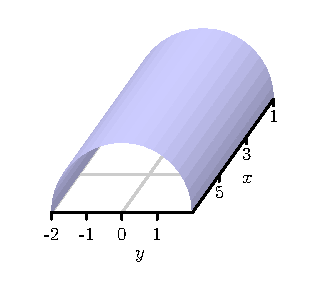
\includegraphics{figures/fig_11_1_cylinder.eps}
        \end{center}
        \captionof{figure}{Graph of $f(x,y) =  \sqrt{4-y^2}$ on $R$.}
        \label{F:11.1.DI_example}
      \end{minipage}
    \end{center}
  \end{figure}

  \begin{itemize}
    \item Apply the Midpoint Rule to estimate the volume between the graph
      $z=f(x,y)$ and the $xy$-plane.  
    \item Compare this to the exact volume computed using simple
      geometry.
    \end{itemize}

    \ea

\end{activity}


\aftera
